\documentclass[titlepage]{scrartcl}
\usepackage{enumitem}
\usepackage[british]{babel}
\usepackage[style=apa, backend=biber]{biblatex}
\DeclareLanguageMapping{british}{british-apa}
\usepackage{url}
\usepackage{float}
\usepackage[labelformat=empty]{caption}
\restylefloat{table}
\usepackage{perpage}
\MakePerPage{footnote}
\usepackage{abstract}
\usepackage{graphicx}
% Create hyperlinks in bibliography
\usepackage{hyperref}
\usepackage{amsmath}

\usepackage[T1]{fontenc}
\usepackage[utf8]{inputenc}
\usepackage{blindtext}
\setkomafont{disposition}{\normalfont\bfseries}

\graphicspath{
    {./resources/},
}
\addbibresource{~/Documents/library.bib}
\DeclareSourcemap{
    \maps{
        \map{ % Replaces '{\_}', '{_}' or '\_' with just '_'
            \step[fieldsource=url,
                  match=\regexp{\{\\\_\}|\{\_\}|\\\_},
                  replace=\regexp{\_}]
        }
        \map{ % Replaces '{'$\sim$'}', '$\sim$' or '{~}' with just '~'
            \step[fieldsource=url,
                  match=\regexp{\{\$\\sim\$\}|\{\~\}|\$\\sim\$},
                  replace=\regexp{\~}]
        }
    }
}

\newsavebox{\abstractbox}
\renewenvironment{abstract}
  {\begin{lrbox}{0}\begin{minipage}{\textwidth}
   \begin{center}\normalfont\sectfont\abstractname\end{center}\quotation}
  {\endquotation\end{minipage}\end{lrbox}%
   \global\setbox\abstractbox=\box0 }

\usepackage{etoolbox}
\makeatletter
\expandafter\patchcmd\csname\string\maketitle\endcsname
  {\vskip\z@\@plus3fill}
  {\vskip\z@\@plus2fill\box\abstractbox\vskip\z@\@plus1fill}
  {}{}
\makeatother

\DeclareCiteCommand{\citeyearpar}
    {}
    {\mkbibparens{\bibhyperref{\printdate}}}
    {\multicitedelim}
    {}

% MATLAB Code block stuff...
\usepackage{color}
\usepackage{listings}

\definecolor{dkgreen}{rgb}{0,0.6,0}
\definecolor{gray}{rgb}{0.5,0.5,0.5}

\lstset{language=Matlab,
   keywords={break,case,catch,continue,else,elseif,end,for,function,
      global,if,otherwise,persistent,return,switch,try,while},
   basicstyle=\ttfamily,
   keywordstyle=\color{blue},
   commentstyle=\color{gray},
   stringstyle=\color{dkgreen},
   numbers=left,
   numberstyle=\tiny\color{gray},
   stepnumber=1,
   numbersep=10pt,
   backgroundcolor=\color{white},
   tabsize=4,
   showspaces=false,
   showstringspaces=false}

\begin{document}
\title{ECS731U/P --- Music Analysis and Synthesis}
\subtitle{\LARGE{Assignment 3 Report}}
\author{Sam Perry --- EC16039}

\maketitle

\section{Task Solution}
The approach to this task consisted of the extraction of relevant features from
the audio, the estimation of stable sections from these features, the
refinement of segment boundaries and finally, the synthesis of the output audio
based on the best segment found.

\subsection{Feature extraction}
Three features were chosen as measurements for the overall stability at any
time in the audio. These features are fundamental frequency ($f_0$), Root Mean
Square and Spectral Flux.\\
Spectral flux, used for measuring salience of spectral content, was calculated as:
$$
\text{SF}(n) =
\frac{\sqrt{\sum_{K/2-1}^{k=0}(|X(k,n)|-|X(k,n-1)|)^2}}{K/2}
$$
where $X$ represents the DFT of the audio, $K$ is the current DFT bin index, $K$ is
the total number of bins and $n$ is the current sample
index~\parencite{Lerch2012}.\\
RMS was chosen as a simple measure for loudness and was calculated as:
$$RMS(n) = \sqrt{\frac{1}{N}\sum_{i=i_s(n)}^{i_e(n)}{x(i)^2}}$$
where $i$ represents indexes in the current frame of audio and $N$ is the total
number of indexes in the current frame~\parencite{Lerch2012}.

An implementation of the YIN algorithm was adapted for fundamental frequency
estimation~\parencite[p352-353]{Zolzer2011}. This implementation was further
modified to use parabolic interpolation for increased accuracy.
It was also noticed that as the system would only be analysing audio of
specific, relatively static pitches, it was not necessary to differentiate
between octaves. For this reason, the $f_0$ was wrapped and centred
using the chroma spectrum~\parencite[p.4]{Peeters2006} This allowed for the negation of octave errors
commonly seen in auto-correlation based $f_0$ estimation algorithms. This was
achieved by first mapping estimated frequencies to the semi-tone pitch
spectrum:
$$n(f_k) = 12\log_2\Big(\frac{f_k}{440}\Big)+69$$
Pitches were then wrapped around a single octave and centred on the spectrum by
subtracting the median and adding half an octave:
$$c(n) = \bmod((n-\mu)+6, 12)$$
where $f_k$ is the current frequency estimate, $n$ is the current estimate
mapped to the semi-tone pitch spectrum and $\mu$ is the median of all $n$.
This significantly improved the measurement of pitch spread  as discussed in
the following section.
Illustration of normalised feature values for a single guitar note can be seen
in figure~\ref{Guitar14RawFeatures}

\subsection{Feature analysis/loop selection}
Having extracted relevant features, analysis is then performed to determine the
stability of the audio.  A moving standard deviation is taken for each of the
three features, creating 3 vectors to measure the spread of these features over
time.  An iteratively increasing threshold is then applied to the standard
deviation measurements, searching for segments of consecutive frames to be used
for looping. A frame is considered viable if it's length was greater than it's
mean fundamental period multiplied by the minimum number of periods set as a
parameter. From these viable frames, the frame with the lowest accumulated
average standard deviation is chosen to be the best match. An example of
segmentation based on standard deviation values is illustrated in
figure~\ref{Guitar14StdDevSeg}.\\
Upon finding a suitable frame, positive zero crossings are searched for around
it's starting index and the closest multiple to the mean $f_0$ period at the end
point. This was to implemented to account for inaccuracies in estimation of the
segment's pitch and to help ensure an integer number of periods were selected
for a segment. These values form the final start and end indexes for the loop.
Segmentation of audio based on zero-crossing is illustrated in
figure~\ref{ZeroX}

\subsection{Synthesis}
Output is then synthesized by segmenting the audio into three sections (start,
loop and end) and inserting an integer number of loops in place of
the loop segment found. The number of loops inserted is calculated based on the
duration provided in samples, and the closest number of loops to the desired
overall length of the sample is used.
Initially a method using overlap-add with crossfading was tested. However, this
was eventually discarded as it was decided that the amplitude modulation
created detracted significantly from the overall quality of output.

\section{Evaluation}
The system was evaluated by increasing the duration of a selection of single
note samples (original samples included in \texttt{./src/media}). It was
assumed for the purpose of evaluation, that the system would be used for
increasing single note durations of harmonic instruments for use in software
samplers, for example. It is likely that the system would not perform well on
polyphonic recordings of percussive instruments.\\
The minimum period allowed for a viable segment proved to be the primary
parameter used for tuning the system.  Low values resulted in the selection of
smaller loops, with less variation in content over time. Too small, and the
loop would sound synthetic without variation. High values resulted in larger
loops with more variation. Higher variation clearly sounded more natural but
increased the chance of discontinuities due to sudden changes at loop points.
Careful splicing of samples at zero crossings ensured smooth transitions at
loop points.  However, long samples will evolve over time, thus inherently not
looping well due to the lack of continuity between the segment's start and
finish. Reasonable values of 14-25 periods were found to provide a good trade off
between these two characteristics.\\
A range of audio files were tested using the system. Each was stretched by a
duration of 1.5 time it's original duration. This was the only duration tested
significantly as the system is not designed to handle anything less than the
original duration of the sample and further durations would simply add more
loops.\\
Instruments with the least variation in amplitude and spectral content over
time (such as the trumpet and trombone) appeared to perform best, with only
minor variations in amplitude noticeably missing from the looped section.
Across the range of samples, it was clear that vibrato posed a key problem
with this style of synthesis. This was particularly clear in the cello results,
as looped segments did not preserve the oscillations of the vibrato, creating a
clearly synthetic loop. This would need to be addressed, possibly by segmenting
based on multiples of the vibrato's period in addition to the frequency.\\
Vocal vibrato performed the worst of all samples. This was entirely expected as
statically looping audio with such temporal and spectral variation throughout
will result in clearly unnatural results.\\
Other instruments that have clear decays, such as the piano and guitar, were
synthesized to a reasonable degree with correct selection of the minimum
period. The most noticeable effect was in the sudden sustain of the note. This
is obviously not possible with these types of instruments in the real-world so
would unavoidably sound unnatural. For this reason, these are perhaps less
useful examples for demonstration of this system. However, they do loop
relatively smoothly.

\subsection{Known bugs}
At present there is only one clear know bug with the system, having tested using a
selection of reasonable inputs. If the minimum periods is set so low that
zero-crossing selection of start and end times converge on the same point, this
may not be handled correctly by the system in all cases. This is an edge case
that is unlikely to occur.
It is also noted that returned audio from \texttt{loop(signal, duration,
loopPoints, p)} may not be of the exact duration specified as an argument in
samples. This is due to the closest integer multiple of loops having been used.
This is considered a caveat rather than a bug as it is expected and does not
have a significantly negative impact on the system.
Further testing is required to determine any further problems that have been
missed due to the relatively fast design and implementation process. 

\subsection{Possible improvements}
Given more time for development, a number of further improvements to the system
could be implemented to improve overall performance:
\begin{itemize}
    \item The parametrisation of moving standard deviation window size could
        be tested and would likely yield variations in segment selection
    \item The use of varying analysis window sizes was not tested, and other
        window sizes than the 2048 default may also benefit results.
    \item It is not guaranteed that the start and end segment indexes mark
        start/end points of periods of the signal (Despite a reasonable amount
        of effort to ensure this). Further research would need to be undertaken
        into ways of improving the selection of these indexes.
    \item Currently, threshold are applied to all features at set increments.
        The testing between incrementation of each feature may offer more
        precise classification of frames on each iteration. Gradient ascent
        could also be applied for accurate and more efficient calculation of
        segments.
    \item Further improvements could be made in an attempt to deal with the
        effects of vibrato. Providing a further feature for this may aid in the
        segmentation of audio.
\end{itemize}

\section{Figures}
\begin{figure}[H]
    \caption{Raw normalised feature values and segmentation (minimum period
    length = 14)}
    \makebox[\textwidth]{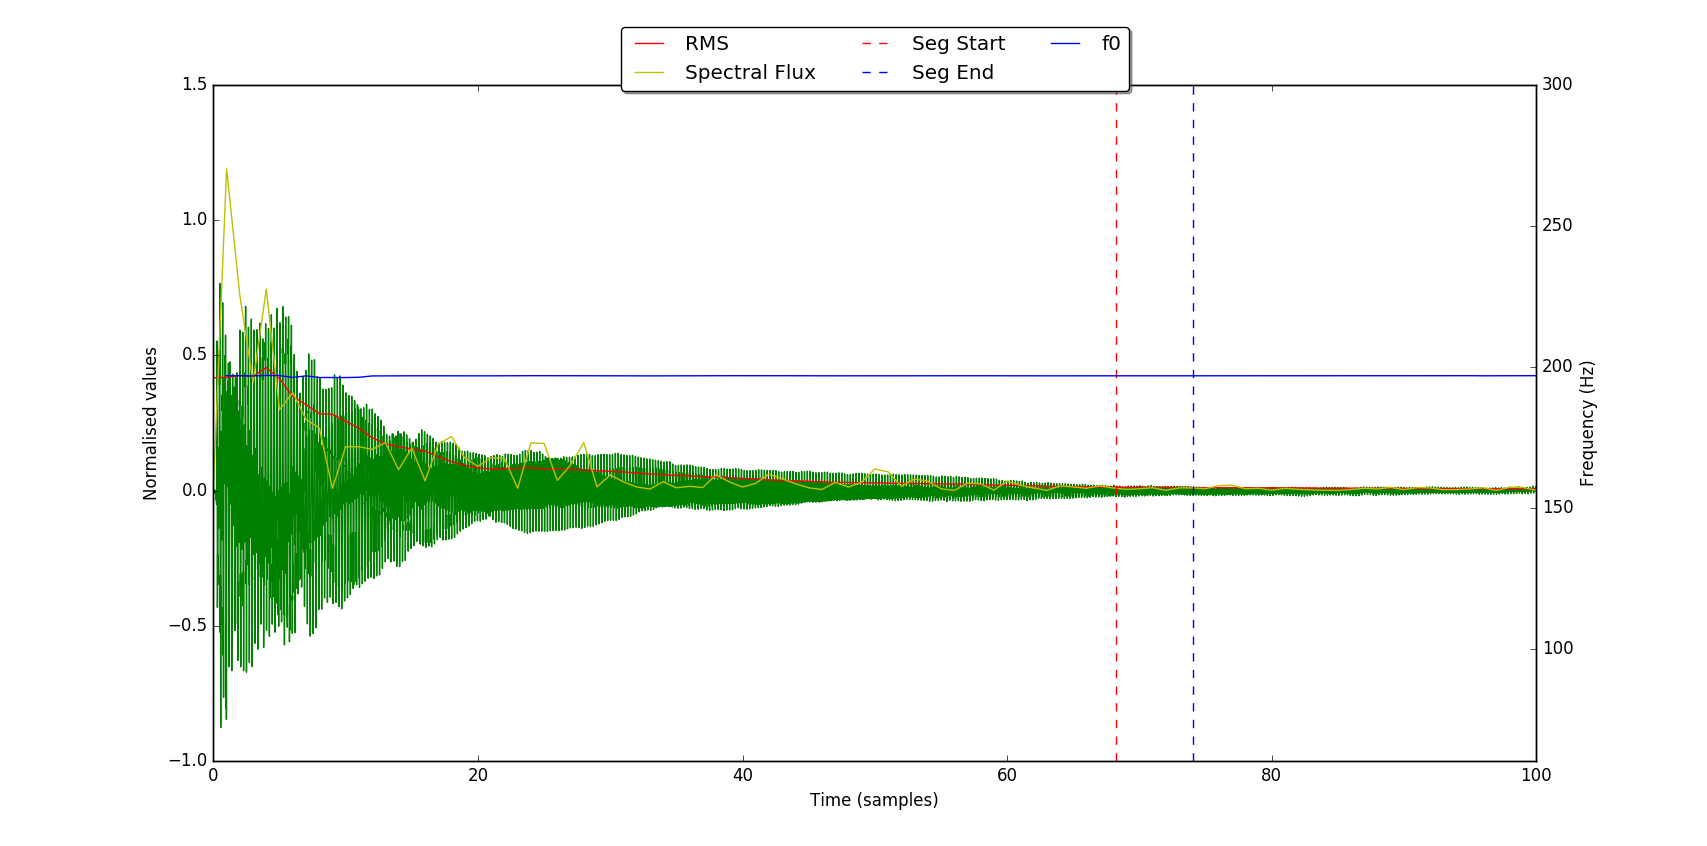
\includegraphics[width=1.2\textwidth]{Guitar14RawFeatures}}
    \label{Guitar14RawFeatures}
\end{figure}
\begin{figure}[H]
    \caption{Standard deviation of features and segment selection (minimum period
    length = 14)}
    \makebox[\textwidth]{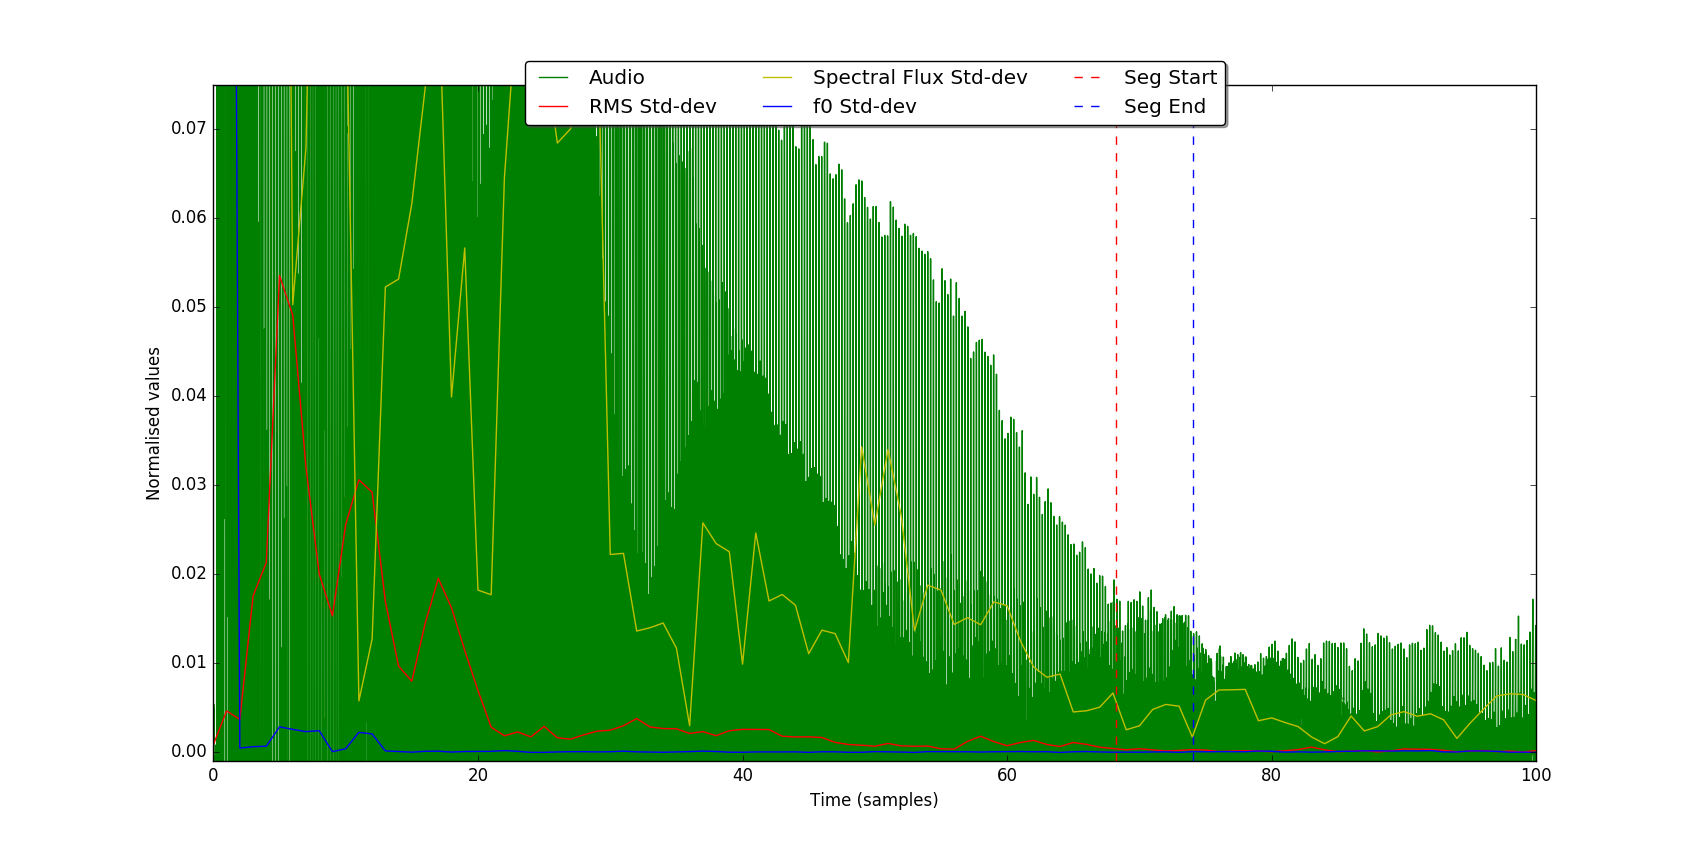
\includegraphics[width=1.2\textwidth]{Guitar14StdDevSeg}}
    \label{Guitar14StdDevSeg}
\end{figure}
\begin{figure}[H]
    \caption{Zero-crossing segmentation of audio (Minimum period length = 3)}
    \makebox[\textwidth]{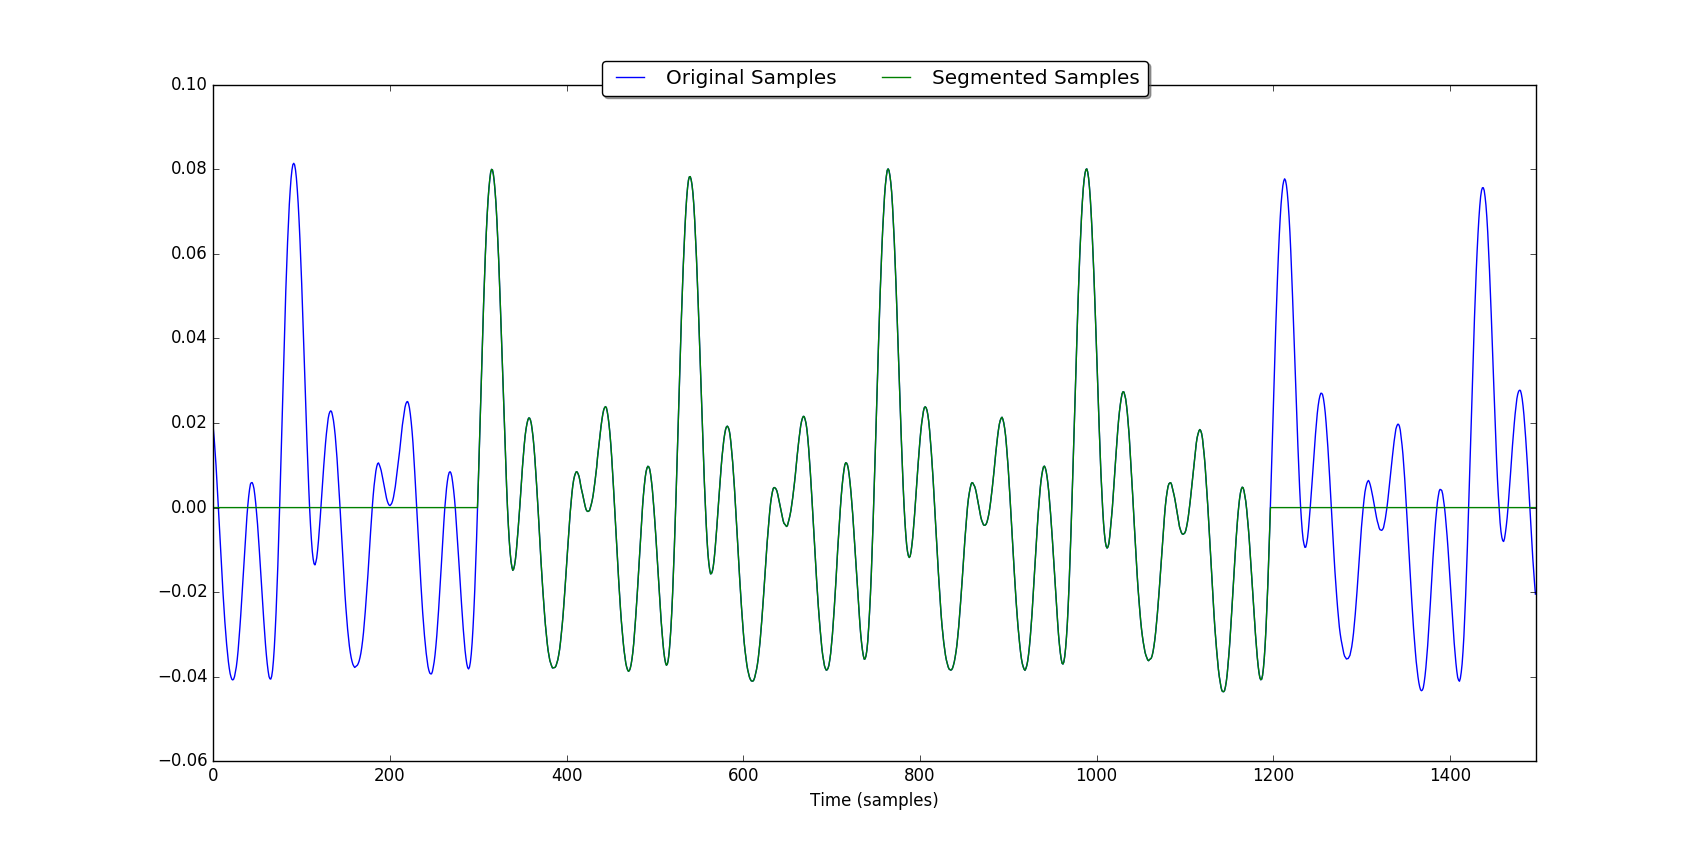
\includegraphics[width=1.2\textwidth]{ZeroX}}
    \label{ZeroX}
\end{figure}

\printbibliography

\end{document}
